\documentclass[default]{beamer}
\setbeamertemplate{navigation symbols}{}

\usetheme{CambridgeUS}
\useoutertheme{infolines}
%\usecolortheme{crane}

\usepackage{cmap}	% Поддержка поиска русских слов в PDF (pdflatex)
\usepackage[T2A]{fontenc}       %поддержка кириллицы
\usepackage[utf8]{inputenc}	% Выбор языка и кодировки
\usepackage[english, russian]{babel}

\usepackage{color}
\usepackage{listings}

\graphicspath{{../../images/oop/}} 			% Пути к изображениям

\makeatletter
\setbeamertemplate{footline}
{
	\leavevmode%
	\hbox{%
		\begin{beamercolorbox}[wd=.333333\paperwidth,ht=2.25ex,dp=1ex,center]{author
				in head/foot}%
			\usebeamerfont{author in
				head/foot}\insertshortauthor~~\beamer@ifempty{\insertshortinstitute}{}{(\insertshortinstitute)}
		\end{beamercolorbox}%
		\begin{beamercolorbox}[wd=.333333\paperwidth,ht=2.25ex,dp=1ex,center]{title in
				head/foot}%
			\usebeamerfont{title in head/foot}\insertshorttitle
		\end{beamercolorbox}%
		\begin{beamercolorbox}[wd=.333333\paperwidth,ht=2.25ex,dp=1ex,right]{date in
				head/foot}%
			\usebeamerfont{date in head/foot}\insertshortdate{}\hspace*{2em}
			\insertframenumber{}\hspace*{2ex} 
		\end{beamercolorbox}
	}%
	\vskip0pt%
}

\definecolor{mygreen}{rgb}{0,0.6,0}
\definecolor{mygray}{rgb}{0.9,0.9,0.9}
\definecolor{mymauve}{rgb}{0.58,0,0.82}
\lstset{
	backgroundcolor=\color{mygray},   % choose the background color
	basicstyle=\footnotesize,        % size of fonts used for the code
	breakatwhitespace=true,			 % sets if automatic breaks should only happen at whitespace
	breaklines=true,                 % automatic line breaking only at whitespace
	commentstyle=\color{mygreen},    % comment style
	escapeinside={\%*}{*)},          % if you want to add LaTeX within your code
	keepspaces=true,                 % keeps spaces in text, useful for keeping indentation of code (possibly needs columns=flexible)
	keywordstyle=\color{blue},       % keyword style
	stringstyle=\color{mymauve},     % string literal style
	showspaces=false,                % show spaces everywhere adding particular underscores; it overrides 'showstringspaces'
	showstringspaces=false,          % underline spaces within strings only
	showtabs=false,					 % show tabs within strings adding particular underscores
	tabsize=4,                       % sets default tabsize to 2 spaces
}

\setbeamertemplate{bibliography entry title}{}
\setbeamertemplate{bibliography entry location}{}
\setbeamertemplate{bibliography entry note}{}

\begin{document}
	
	\title[ООП. Лабораторные]{Основы объектно"--~ориентированного программирования.
		Лабораторные}
	\author[Панов]{Александр Панов}
	\institute[МФТИ]{Московский физико-технический институт}
	\date{февраль 2015 г.} 
	
	\begin{frame}
		\titlepage
	\end{frame}
	
	\section {Семинар 1}
	
	\begin{frame}
		\frametitle{Цели курса}
		
		\begin{itemize}
			\item Освоить идеологию объектно"--~ориентированного программирования.
			\item Понять принципы программирования структур данных и типовых решений
			(patterns).
			\item Научиться писать программы на объектно"--~ориентированном языке (Java,
			C++, Python).
			\item Начать создавать безопасные и легко понимаемые программы.
			\item Научиться работать в команде с использованием средств командной
			разработки кода.
			\item Освоить основы параллельного программирования.
			\item Начать пользоваться стандартными и сторонними библиотеками для решения
			своих задачах.
			\item Овладеть инструментами компиляции, отладки и сборки сложных программ.
		\end{itemize}
	\end{frame}
	
	\begin{frame}
		\frametitle{Работа в семестре}
		
		\begin{itemize}
			\item Сформировать команды минимум по 3 человека, максимум "--- 5 (конец
			февраля).
			\item Определиться с языком программирования в команде и темой курсового
			проекта (конец февраля).
			\item Подготовить презентацию своего проекта (конец марта).
			\item Выполнить две семестровых задачи (конец марта).
			\item Сдать курсовой проект (май).
		\end{itemize}
		
		\par\bigskip
		Среда разработки и система контроля версий "--- по своему усмотрению.
	\end{frame}
	
	\begin{frame}
		\frametitle{Литература}
		
		\bibliographystyle{gost2008p}
		\nocite{*}
		\inputencoding{cp1251}
		\bibliography{../../biblio/misc}
		\inputencoding{utf8}
	\end{frame}
			
	\begin{frame}
		\frametitle{TIOBE Index}
		
		Индекс, оценивающий популярность языков программирования. Основан на подсчёте
		результатов поисковых запросов, содержащих название языка (Google, Blogger,
		Wikipedia, YouTube, Baidu, Yahoo!, Bing, Amazon).
		http://www.tiobe.com/index.php/content/paperinfo/tpci/index.html
		
		\begin{columns}
			\begin{column}{0.5\textwidth}
				\begin{figure}
					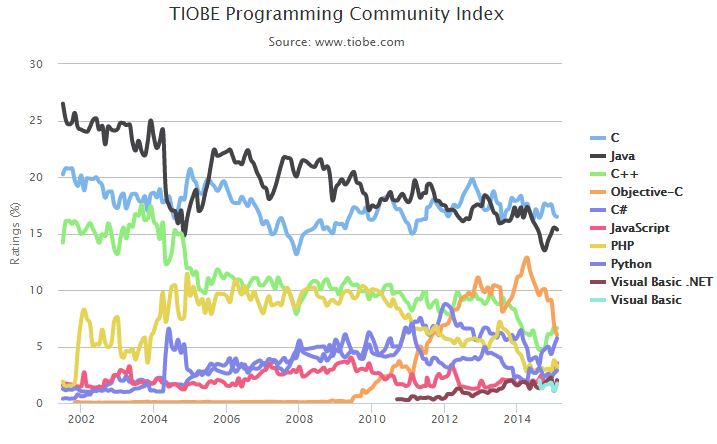
\includegraphics[width=0.8\textwidth]{tiobe_graph}
				\end{figure}
			\end{column}
			\begin{column}{0.5\textwidth}
				\begin{figure}
					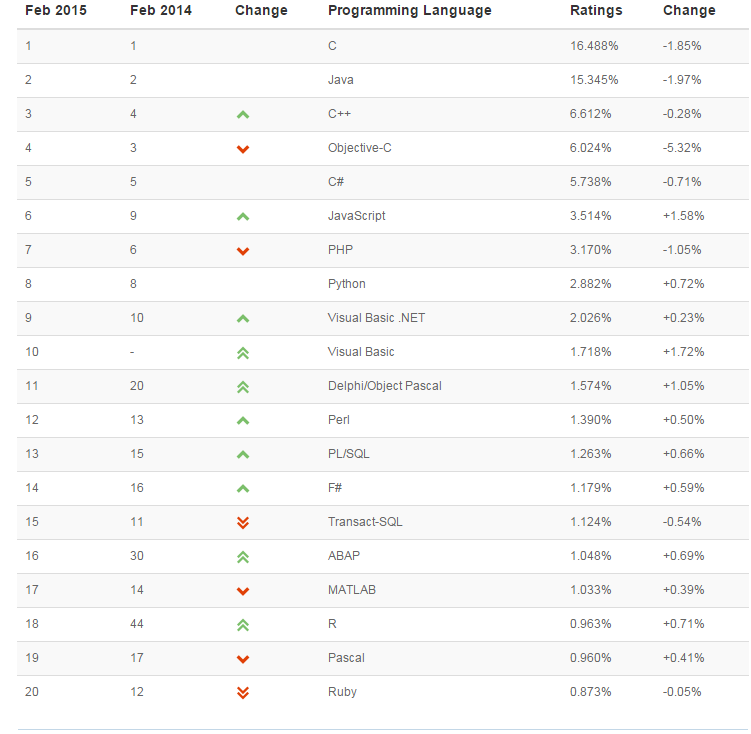
\includegraphics[width=0.8\textwidth]{tiobe_table}
				\end{figure}
			\end{column}	
		\end{columns}
	\end{frame}
	
	\begin{frame}
		\frametitle{ООП на примере языка C++}
		
		\begin{itemize}
			\item История с 1980~г.: изначально <<C with classes>>, крайняя версия "---
			C++11.
			\item Стандартизация с 1996~г. 
			\item Ключевая особенность "--- полная совместимость с C.
			\item Высокая производительность.
			\item Наличие совместимости с C приводит к путанице при использовании
			устаревших функций.
			\item Большое количество библиотек, в том числе и с дублирующими функциями.
		\end{itemize}		
	
	\end{frame}
	
	\begin{frame}
		\frametitle{ООП на примере языка Java}
		
		\begin{itemize}
			\item История с 1995~г.: 6 версий "--- крайняя JDK 1.8.
			\item Поддержка Sun"--~Oracle http://docs.oracle.com/javase/8/docs/
			\item Ключевая особенность "--- программы транслируются в байт-код,
			выполняемый виртуальной машиной Java (JVM). JVM реализована для всех типов
			операционных систем.
			\item Облегченное управление памятью "--- сборка мусора garbage collector
			(GC).
			\item Программные стеки: JavaSE (desktop"--~приложения), JavaEE
			(web"--~приложения), JavaFX (rich"--~приложения), Android (мобильные
			приложения).
			\item Богатый набор уже написанного кода и большое количество библиотек и
			фреймворков (frameworks), решающих огромное количество задач.
		\end{itemize}
	\end{frame}
	
	\begin{frame}
		\frametitle{Компоненты языка Java}
		
		\begin{figure}
			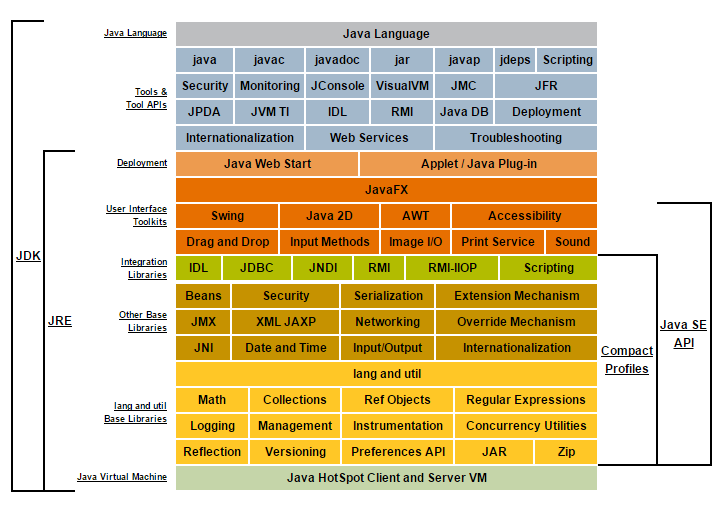
\includegraphics[width=0.8\textwidth]{java_stack}
		\end{figure}
	\end{frame}	
	
	\begin{frame}
		\frametitle{Инструменты языка C++}
		
		\begin{itemize}
			\item STandart Library (STL) "--- библиотека шаблонов.
			\item Boost "--- одна из самых известных библиотек инструментов.
			\item make "--- инструмент сборки программ.
			\item gdb "--- инструмент отладки.
		\end{itemize}
	\end{frame}	

\defverbatim[colored]\lstA{%
\begin{lstlisting}[language=java]
double a = 1, b = 1, c = 6; 
double D = b * b - 4 * a * c; 
if (D >= 0) { 
	double x1 = (-b + Math.sqrt (D)) / (2 * a);
	double x2 = (-b - Math.sqrt (D)) / (2 * a); 
}

int x = 2; 
int y = 0; 
/* if (x > 0) 
		y = y + x*2; 
	else 
		y = -y - x*4; */ 
y = y*y;// + 2*x;
\end{lstlisting}
}
	\begin{frame}
		\frametitle{Примеры на Java}
		
		\lstA
	\end{frame}
	
\defverbatim[colored]\lstB{%
\begin{lstlisting}[language=java]
public class Demo { 

	public static void main (String args[]) {
		System.out.println("Hello, world!");
	}
}
\end{lstlisting}
}

	\begin{frame}
		\frametitle{Hello World! на Java}
		\lstB
		
		\par\bigskip
		Команда компиляции "--- javac Demo.java
		
		Команда запуска скомпилированного приложения "--- java Demo
	\end{frame}
	
	\begin{frame}
	\frametitle{Лексика языка}
	
	\begin{itemize}
		\item Идентификаторы "--- это имена,~которые даются различным элементам языка
		для упрощения доступа к ним. Имена имеют пакеты, классы, интерфейсы, поля,
		методы, аргументы и локальные переменные.
		\item Ключевые слова "--- это зарезервированные слова, состояшие из
		ASCII"--~символов и выполняющие различные задачи языка: abstract, double, int,
		class, public, void и т.~п.
		\item Литералы позволяют задать в программе значения для числовых, символьных и строковых выражений, а также null"--~литералов.
		\item Операторы используются в различных операциях "--- арифмтеических, логических, битовых, опреациях сравнения и присваивания: =, ==, >, <, +, - и т.~п.
	\end{itemize}
	\end{frame}


\defverbatim[colored]\lstC{%
\begin{lstlisting}[language=bash]
ping 64.0.0.0 -c 2 -w2 || wget -qO - "login.telecom.mipt.ru/bin/login.cgi?login=LOGIN &memorize=on&password=
$((wget login.telecom.mipt.ru/bin/getqc.cgi -qO -; echo -n PASSWORD) | md5sum - | head -c32)"
\end{lstlisting}
}	
	\begin{frame}
		\frametitle{Интернет на виртуальных контейнерах}
		\lstC
	
	\end{frame}
	
	%	\begin{frame}
	%		\frametitle{Цели курса}
	%		
	%		\begin{itemize}
	%			\item
	%		\end{itemize}
	%	\end{frame}
	
\end{document}
	
	
